\documentclass{article}
\usepackage{amsmath, amssymb, tikz, graphicx, xcolor}
\usepackage[margin=1in]{geometry}
\usepackage{hyperref}
\usepackage{caption}
\usepackage{mathtools}
\usepackage{xcolor}
\usepackage{braket}
\usepackage{ulem}
\usepackage{cancel}
\usepackage{graphicx}
\usepackage{mathtools}
\usepackage{amsmath}  
\usepackage{amsfonts} 
\usepackage{graphicx}
\usepackage{amssymb} 
\usepackage{amsmath}
\usepackage{mathrsfs}
\usepackage{empheq}
\usepackage{amsthm}
 \usepackage{braket}
 \usepackage{amsmath}

\title{Exploration of $\mathbb{Z}_2$ Lattice Gauge Theories -Monte Carlo Simulations}
\author{Hariprashad Ravikumar\\
Under the guidance of Dr. Michael Engelhardt \\
Department of Physics, New Mexico State University \\}

\date{December 2022}

\begin{document}

\maketitle
\begin{center}
\section*{Project Summary}
\end{center}
This project presents a Python-based simulation framework for investigating $\mathbb{Z}_2$ lattice gauge theories using Monte Carlo methods. It employs Metropolis algorithms to explore phase transitions and gauge field dynamics in various dimensional systems. The work integrates numerical modeling, statistical mechanics, and high-performance computation to extract physical observables such as Wilson loops $\langle W \rangle$ and benchmark them against analytical results. The code base demonstrates applied skills in stochastic sampling, scientific programming, and algorithmic implementations, relevant to domains such as computational physics, data-driven modeling, and probabilistic inference.



\tableofcontents

\section{$\mathbb{Z}_2$ lattice gauge theory}
Consider the gauge group $\mathbb{Z}_2$, and define $U_{ij}\in \mathbb{Z}_2$, where $U_{ij}$ is $\pm1$. 
\begin{align}
    U_{ij}&=P.O.\left(\exp{\left(ig_0\int_{x_i}^{x_j}A_{\mu}.dx_{\mu}\right)}\right)
\end{align}
All the following definitions are true even for a general gauge group $G$, and $U_{ij}\in G$, where $U_{ij}$ is an $n\times n$ unitary matrix.
The action should be a sum over all elementary squares of the lattice, where each of these squares or 'plaquettes' is the trace of the product of the group elements surrounding the plaquette
\begin{align}
     S=\sum_\Box S_\Box=\sum_\Box \beta\left[1-\left(\frac{1}{n}\right)Re~Tr\left(U_{ij}U_{jk}U_{kl}U_{li}\right)\right]
\end{align}
\begin{center}
\begin{tikzpicture}[scale=1]
  % Define lattice points in red
  \foreach \x in {0, 1, 2, 3}
    \foreach \y in {0, 1, 2, 3}
      \fill[red] (\x, \y) circle (0.1);
\draw[|<->|, gray] (0.1, 0.1) -- (0.9, 0.1);
\node at (0.5, 0.2) {\textcolor{gray}{$a$}};
  % Draw links
  \foreach \x in {0, 1, 2, 3}
    \foreach \y in {0, 1, 2}
      \draw (\x, \y) -- (\x, \y + 1);
  \foreach \x in {0, 1, 2}
    \foreach \y in {0, 1, 2, 3}
      \draw (\x, \y) -- (\x + 1, \y);
 \draw[thick, blue] (1, 1) -- (2, 1) -- (2, 2) -- (1, 2) -- cycle;
 \draw[->, red, dashed] (1, 1) -- (0.65, 0.85);
   \node at (0.5, 0.8) {\textcolor{red}{$x$}};
  % Add labels
  \node at (1.5, 1.5) {$P_{\mu\nu}(x)$};
  % Add x and y axes
  \draw[->] (0, 0) -- (3.5, 0) node[right] {$\mu$};
  \draw[->] (0, 0) -- (0, 3.5) node[above] {$\nu$};
  % Zoom effect
  \draw[magenta, dashed] (1.5, 1.5) circle (0.8);
  \draw[->, magenta, dashed] (2.3, 1.5) -- (5.7, 1.5)
  \draw[thick, blue] (3, 2) -- (3, 3)
  \draw[blue,->, line width=1.5pt] (3, 2.5) -- ++(0,0.1);
   \node at (4.5, 2.5) {\textcolor{blue}{$U_{\nu}(y)=e^{iaA_{\nu}(y)}$}};
   \draw[->, red, dashed] (3, 2) -- (2.6, 2.2)
   \node at (2.5, 2.2) {\textcolor{red}{$y$}};
  % Create a scope for the plaquette on the left side
  \begin{scope}[xshift=6cm]
   \foreach \x in {1, 2}
    \foreach \y in {1, 2}
      \fill[red] (\x, \y) circle (0.1);
    % Create a plaquette
    \draw[magenta, dashed] (1.8, 1.5) ellipse (1.99 and 1.3);
   \draw[thick, blue] (1, 1) -- (2, 1) -- (2, 2) -- (1, 2) -- cycle;
   \draw[blue,->, line width=1.5pt] (1.5, 1) -- ++(0.1,0);
   \draw[blue,<-, line width=1.5pt] (1.5, 2) -- ++(0.1,0);
   \draw[blue,->, line width=1.5pt] (2, 1.5) -- ++(0,0.1);
   \draw[blue,<-, line width=1.5pt] (1, 1.5) -- ++(0,0.1);
   \draw[->, red, dashed] (1, 1) -- (0.65, 0.85)
   \node at (0.5, 0.8) {\textcolor{red}{$x$}};
    % Add a label for the plaquette on the left side
    \node at (1.5, 0.7) {$U_{\mu}(x)$};
    \node at (3, 1.5) {$U_{\nu}(x+\hat{\mu})$};
    \node at (1.5, 2.4) {$U^{\dagger}_{\mu}(x+\hat{\nu})$};
    \node at (0.4, 1.5) {$U^{\dagger}_{\nu}(x)$};
  \end{scope}
\end{tikzpicture}
\end{center}
Then the action will be,
\begin{align}
    S=&\sum_\Box \beta\left[1-\left(\frac{1}{n}\right)Re~Tr\left(U_{12}U_{23}U_{34}U_{41}\right)\right]\\
    =&\sum_\Box \beta\left[1-\left(\frac{1}{n}\right)Re~Tr\left(e^{\left(ig_0\int_{x_\mu_1}^{x_\mu_2}A_{\mu}.dx_{\mu}\right)}e^{\left(ig_0\int_{x_\mu_2}^{x_\mu_3}A_{\mu}.dx_{\mu}\right)}e^{\left(ig_0\int_{x_\mu_3}^{x_\mu_4}A_{\mu}.dx_{\mu}\right)}e^{\left(ig_0\int_{x_\mu_4}^{x_\mu_1}A_{\mu}.dx_{\mu}\right)}\right)\right]\\
    =&\sum_\Box \beta\left[1-\left(\frac{1}{n}\right)Re~Tr\left(exp{\left(ig_0\oint A_{\mu}.dx_{\mu}\right)}\right)\right]\\
    =&\sum_\Box \beta\left[1-\left(\frac{1}{n}\right)Re~Tr\left(exp{\left(ig_0\iint_s (\partial_\mu A_\nu-\partial_\nu A_\mu)ds\right)}\right)\right]\\
    =&\sum_\Box \beta\left[1-\left(\frac{1}{n}\right)Re~Tr\left(exp{\left(ig_0a^2 F_{\mu\nu}\right)}\right)\right]=\sum_\Box \beta\left[1-\left(\frac{1}{n}\right)Tr\left(\cos{\left(g_0a^2 F_{\mu\nu}\right)}\right)\right]
\end{align}
\begin{align}
    S=&\sum_\Box \beta\left[1-\left(\frac{1}{n}\right)\left(Tr(\mathbb{I}_{n\times n})-Tr\left(\frac{g^2_0a^4F^2_{\mu\nu}}{2}\right)+\mathcal{O}(a^8)\right)\right]\\
    =&\sum_\Box \frac{\beta g^2_0}{2n}Tr(F^2_{\mu\nu})a^4+\mathcal{O}(a^6)\\
    S=&\sum_\Box \frac{\beta g^2_0}{2n}\frac{1}{2}Tr(F_{\mu\nu}F_{\mu\nu})a^4+\mathcal{O}(a^6)
\end{align}

Then in the continuum limit $a\longrightarrow0$,
 \begin{align}
     S=& \frac{\beta g^2_0}{2n}\int\frac{1}{2}Tr(F_{\mu\nu}F_{\mu\nu})d^4x+\mathcal{O}(a^6)
 \end{align}
Thus, we obtain the usual gauge theory action if we identify $\beta=\frac{2n}{g_0^2}$.

\section{THE MONTE CARLO METHOD} 
The lattice regularized quantum expectation value of an observable $\mathcal{O}(U_{ij})$ is given by
\begin{align}
    \braket{\mathcal{O}}&=Z^{-1}\int \prod_{ij}dU_{ij}\mathcal{O}(U_{ij})e^{-S(U_{ij},g)},\\
    Z&=\int \prod_{ij}dU_{ij}e^{-S(U_{ij},g)}
\end{align}
\begin{itemize}
    \item  An initial configuration $C^{(1)}$ is stored in the memory of the computer\footnote{Lattice Gauge Theories and Monte Carlo Simulations book by Claudio Rebbi }.        
    \item From $C^{(1)}$ the computer generates a new configuration $C^{(2)}$ which replaces $C^{(1)}$ in the memory, by a stochastic procedure.
    \item Transition probability $p(C\longrightarrow C')$ is defined for the passage between one configuration and the next. 
    \item From $C^{(2)}$, the computer generates a new configuration $C^{(3)}$, and so on, producing eventually a very large number of configurations. 
    \item Probability of encountering any definite configuration $C^(k)$ at larger $k$ steps converges to a distribution proportional to the correct measure factor $e^{-S(C)}$.
    \item Assuming that after $n_0$ steps the probability distribution has come close enough to the correct limiting one, we approximate the exact quantum expectation values by
    \begin{align}
        \braket{\mathcal{O}}=\frac{1}{n}\sum_{k=n_0+1}^{n}\mathcal{O}(C^{(k)})
    \end{align}
    \item The Boltzmann distribution $p(C) \propto e^{-S(C)}$ must be an eigenvector of the probability matrix $p(C \longrightarrow C')$. This is guaranteed if $p$ obeys the detailed balance condition 
    \begin{align}
        \frac{p(C\longrightarrow C')}{p(C'\longrightarrow C)}=\frac{e^{-S(C')}}{e^{-S(C)}}
    \end{align}
    \item The transition matrix $p(C \longrightarrow C')$ is determined in two steps. First a new candidate configuration $C'$ is selected starting from $C$ according to some probability distribution $p_0(C\longrightarrow C')$, satisfying the equality 
    \begin{align}
        p_0(C\longrightarrow C')\Longrightarrow p_0(C'\longrightarrow C)
    \end{align}
    \item The variation in action $\vartriangle S=S(C')-S(C)$ that would be induced by the change is calculated. 
    \item A pseudo-random number is then selected with a uniform probability distribution between 0 and 1, and: 
    \begin{itemize}
        \item if $r < e^{-\vartriangle S}$, the change is accepted — the new configuration in the sequence is C'.
        \item if $r > e^{-\vartriangle S},$ the change is rejected and the new configuration is again C.
    \end{itemize}
    \item In the Metropolis procedure, the transitions $P_0(C\longrightarrow C')$ and $P(C\longrightarrow C')$ can be further qualified, for a gauge system, as $P_0(U_{ji}\longrightarrow U_{ji}')$ and $P(U_{ji}\longrightarrow U_{ji}')$, all other $U_{ji}$ being kept fixed. 
\end{itemize}
\subsection{$2D$ Ising Model}
Below are the results from the implementation of the Monte-Carlo
Metropolis algorithms in $2D$ Ising model:
\begin{equation}
    {\displaystyle H(\sigma )=-\sum _{\langle ij\rangle }J_{ij}\sigma _{i}\sigma _{j}-\mu \sum _{j}h_{j}\sigma _{j},}
\end{equation}
\begin{figure}[h!]
        \centering
        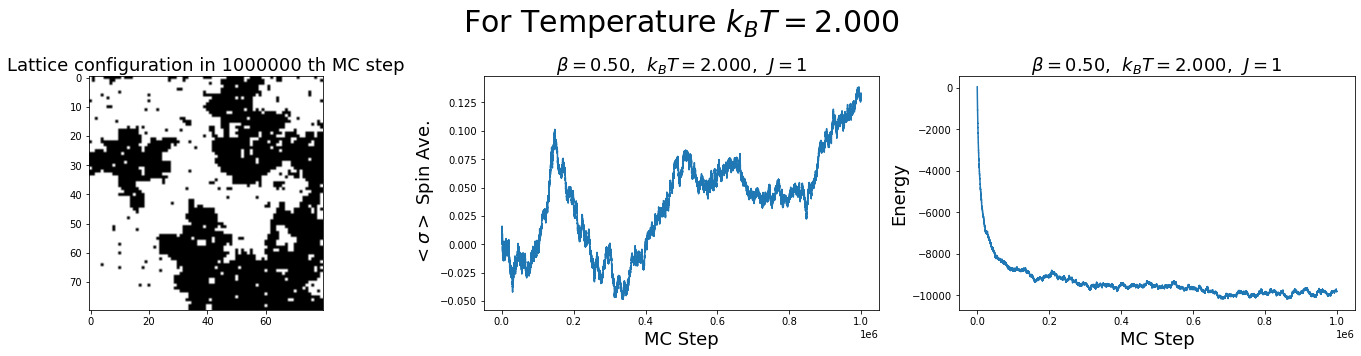
\includegraphics[scale=0.3]{ising2d.png}
    \end{figure}
    \begin{figure}[h!]
        \centering
        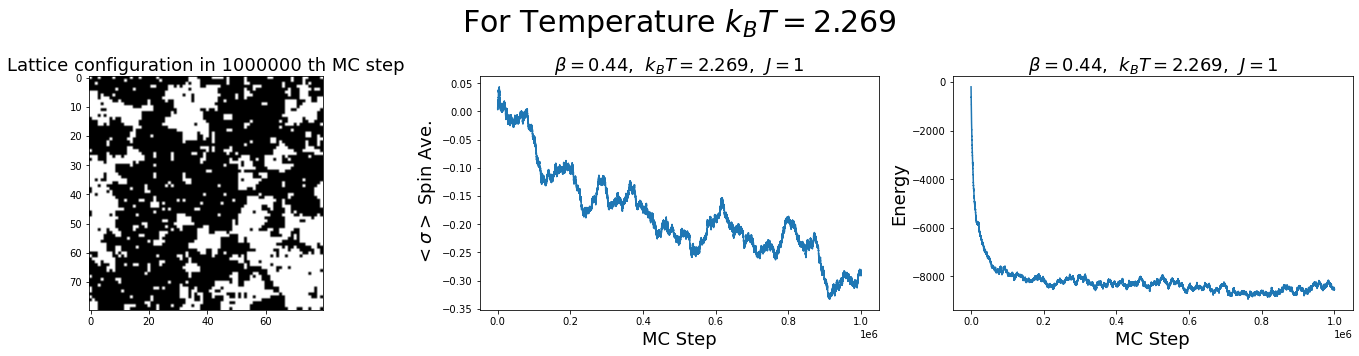
\includegraphics[scale=0.3]{ising2d2.png}
    \end{figure}
    \begin{figure}[h!]
        \centering
        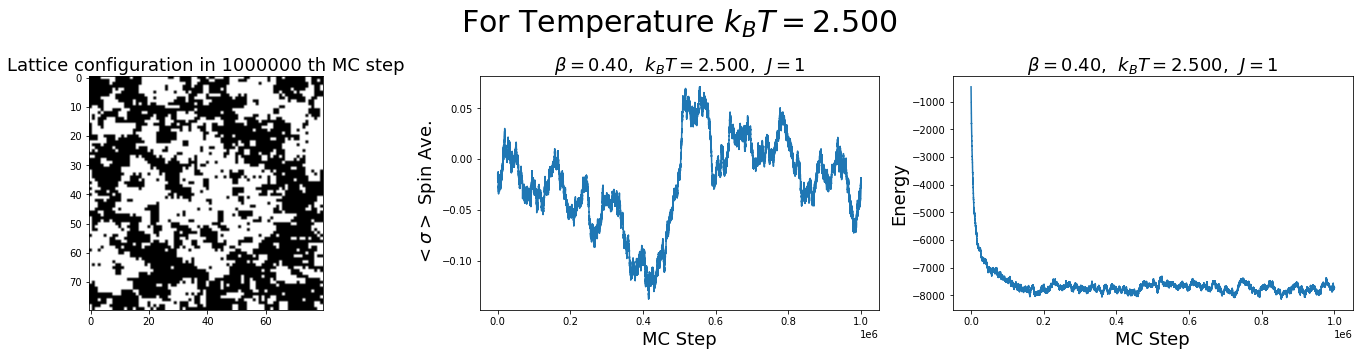
\includegraphics[scale=0.3]{ising2d3.png}
    \end{figure}

\pagebreak
\section{Numerical simulation for Lattice QCD}
    The vacuum expectation value of an observable in a Monte Carlo simulation approximation: (Sum over $U_{n}$ with probability  $\propto e^{-S[U_{n}]}$)
    \begin{align*}
        \boxed{\langle O \rangle =\frac{\int \mathcal{D}[U]e^{-S_{G}[U]}O[U]}{\int\mathcal{D}[U]e^{-S_{G}[U]}}}\rightarrow\boxed{ \langle O \rangle \approx \frac{1}{N}\sum_{U_{n}}O[U_{n}]}
    \end{align*}
    \begin{figure}[h!]
        \centering
        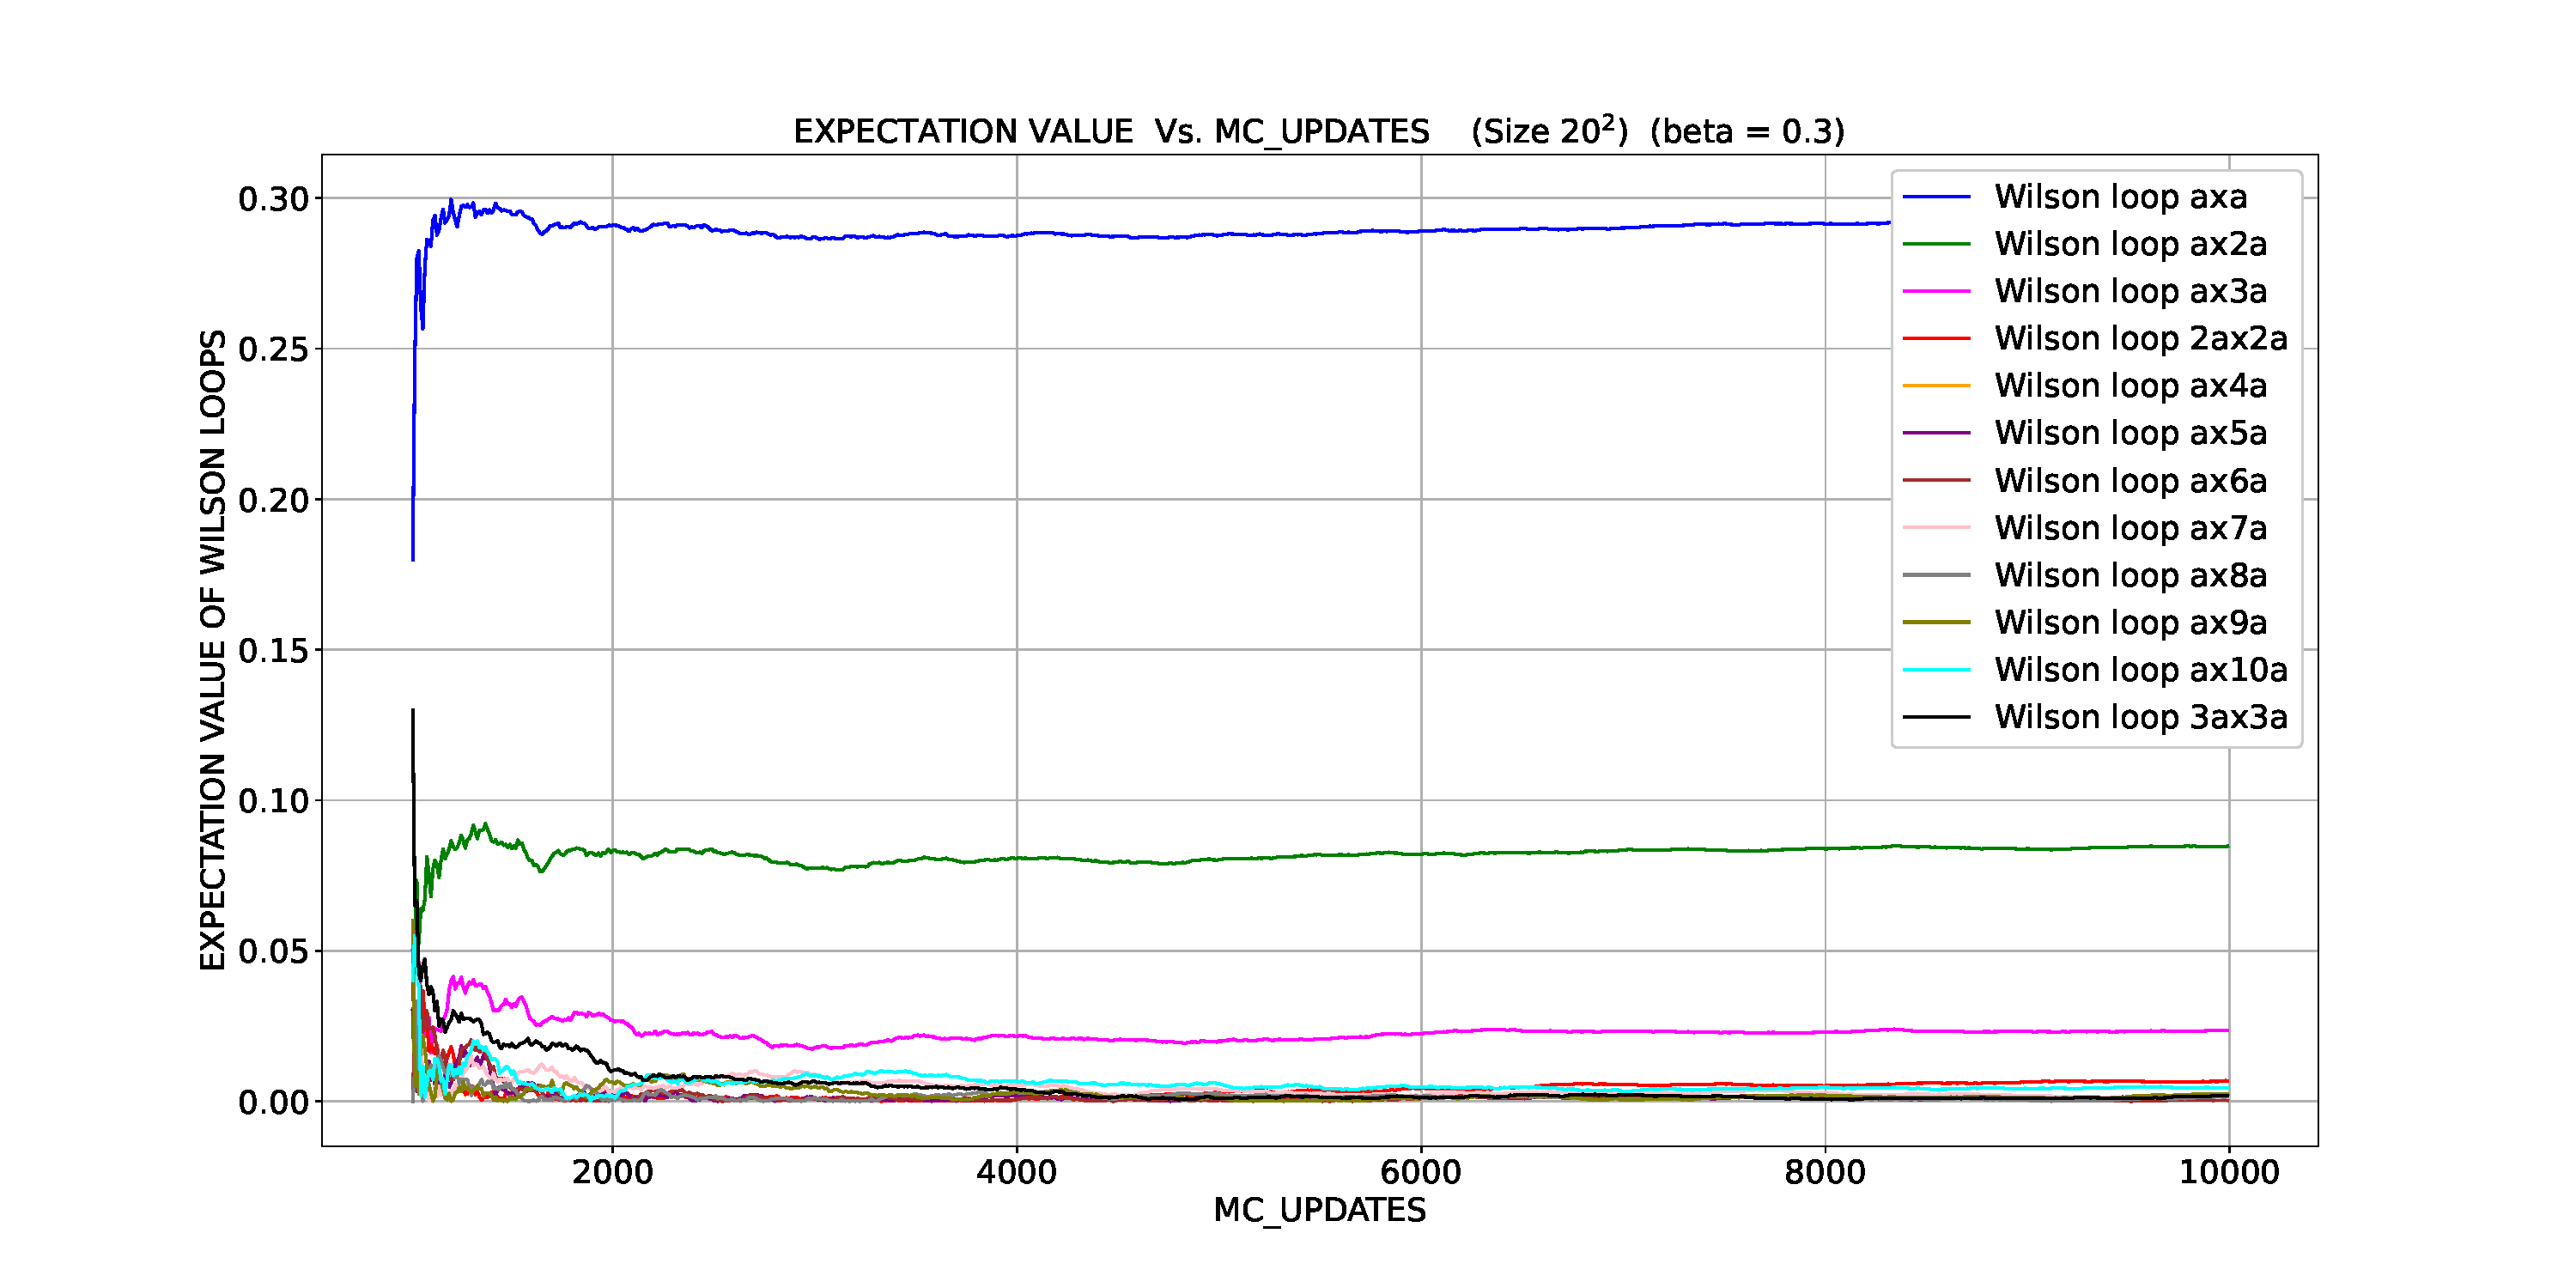
\includegraphics[scale=0.2]{mcstepsz2.pdf}
        \caption{Markov chain - Monte Carlo simulations of $\mathbb{Z}_2$ lattice gauge theory $(1+1)$ }
        \label{fig:enter-label}
    \end{figure}


\subsection{Expectation value of Wilson loop (Analytical solution)} \footnote{An introduction to lattice gauge theory and spin systems, John B. Kogut, Rev. Mod. Phys. 51, 659 – Published 1 October 1979} \footnote{ Gauge Theories of the Strong and Electroweak Interaction by Manfred Böhm, Ansgar Denner, Hans Joos, https://doi.org/10.1007/978-3-322-80160-9}\footnote{Lecture notes, A. Muramatsu- Lattice gauge theory- Summer 2009}
The expectation value of the Wilson loop $\prod_{l\in C} \sigma(l)$ is given by
\begin{align}
    \braket{\prod_{l\in C} \sigma(l)}&=\frac{\int D[\sigma]\prod_{l\in C}\sigma(l)e^{-S}}{\int D[\sigma]e^{-S}}
\end{align}
where, $S=\beta\sum_{P}(1-\sigma(\partial P))$\\
First, the Boltzmann factor for an individual plaquette is calculated, 
\begin{align}
    e^{-\beta(1-\sigma(\partial P))}=e^{-\beta}\cosh{\beta}[1+\sigma(\partial P)\tanh{\beta}]
\end{align}
The expansion of the Boltzmann factor reads 
\begin{align}
    e^{-\beta\sum_{P}(1-\sigma(\partial P))}&=\prod_{P}e^{-\beta}\cosh{\beta}[1+\sigma(\partial P)\tanh{\beta}]\\
    &=(e^{-\beta}\cosh{\beta})^{N^2}\prod_{P}[1+\sigma(\partial P)\tanh{\beta}]\\
    &=(e^{-\beta}\cosh{\beta})^{N^2}\Bigg[[1+\sigma(\partial P_1)\tanh{\beta}][1+\sigma(\partial P_2)\tanh{\beta}]\dots\dots[1+\sigma(\partial P_{N^2})\tanh{\beta}]\Bigg]\\
    &=(e^{-\beta}\cosh{\beta})^{N^2}\Bigg[[1+\tanh{\beta}\left(\sum_{G^{(1)}}\prod_{P\in G^{(1)}}\sigma(\partial P)\right)+\dots+(\tanh{\beta})^{N^2}\left(\sum_{G^{(N^2)}}\prod_{P\in G^{(n^2)}}\sigma(\partial P)\right)]\Bigg]\nonumber\\
    e^{-\beta\sum_{P}(1-\sigma(\partial P))}&=(e^{-\beta}\cosh{\beta})^{N^2}\sum_{n=0}^{N^2}(\tanh{\beta})^{n}\Bigg[\sum_{G^{(n)}}\prod_{P\in G^{(n)}}\sigma(\partial P)\Bigg]
\end{align}
Then the Boltzmann
factor (partition function) is
\begin{align}
    Z &=  \int D[\sigma]e^{-\beta\sum_{P}(1-\sigma(\partial P))}\\
    &=(e^{-\beta}\cosh{\beta})^{N^2}\sum_{n=0}^{N^2}(\tanh{\beta})^{n}\Bigg[\sum_{G^{(n)}}\int D[\sigma]\prod_{P\in G^{(n)}}\sigma(\partial P)\Bigg]
\end{align}
the only non zero term in this sum is when $n=0$, i.e. $G^{(0)}$ empty lattice graph, because,
\begin{align}
    \int D[\sigma]\prod_{P\in G^{(n)}}\sigma(\partial P) = \sum_{\{\sigma \in C\}}\prod_{l\in C}\sigma(l)\sum_{\{\sigma\notin C\}}1 = 0
\end{align}
So,
\begin{align}
Z&=(e^{-\beta}\cosh{\beta})^{N^2}
\end{align}
\\
\\

Now, the numerator,
\begin{align}
    \int D[\sigma]\prod_{l\in C}\sigma(l)e^{-S}&=(e^{-\beta}\cosh{\beta})^{N^2}\sum_{n=0}^{N^2}(\tanh{\beta})^{n}\Bigg[\sum_{G^{(n)}}\int D[\sigma]\prod_{l\in C}\sigma(l)\prod_{P\in G^{(n)}}\sigma(\partial P)\Bigg]
\end{align}
here, only those $G^{(n)}$ that contribute is the one in which $\partial G^{(n)} = C$, this
is a single graph consisting of $Ar[C]$ plaquettes, where $Ar[C]$ is the number
of plaquettes which are enclosed by $C$, i.e. the area enclosed by $C$.
applies. 
\begin{figure}[h!]
    \centering
    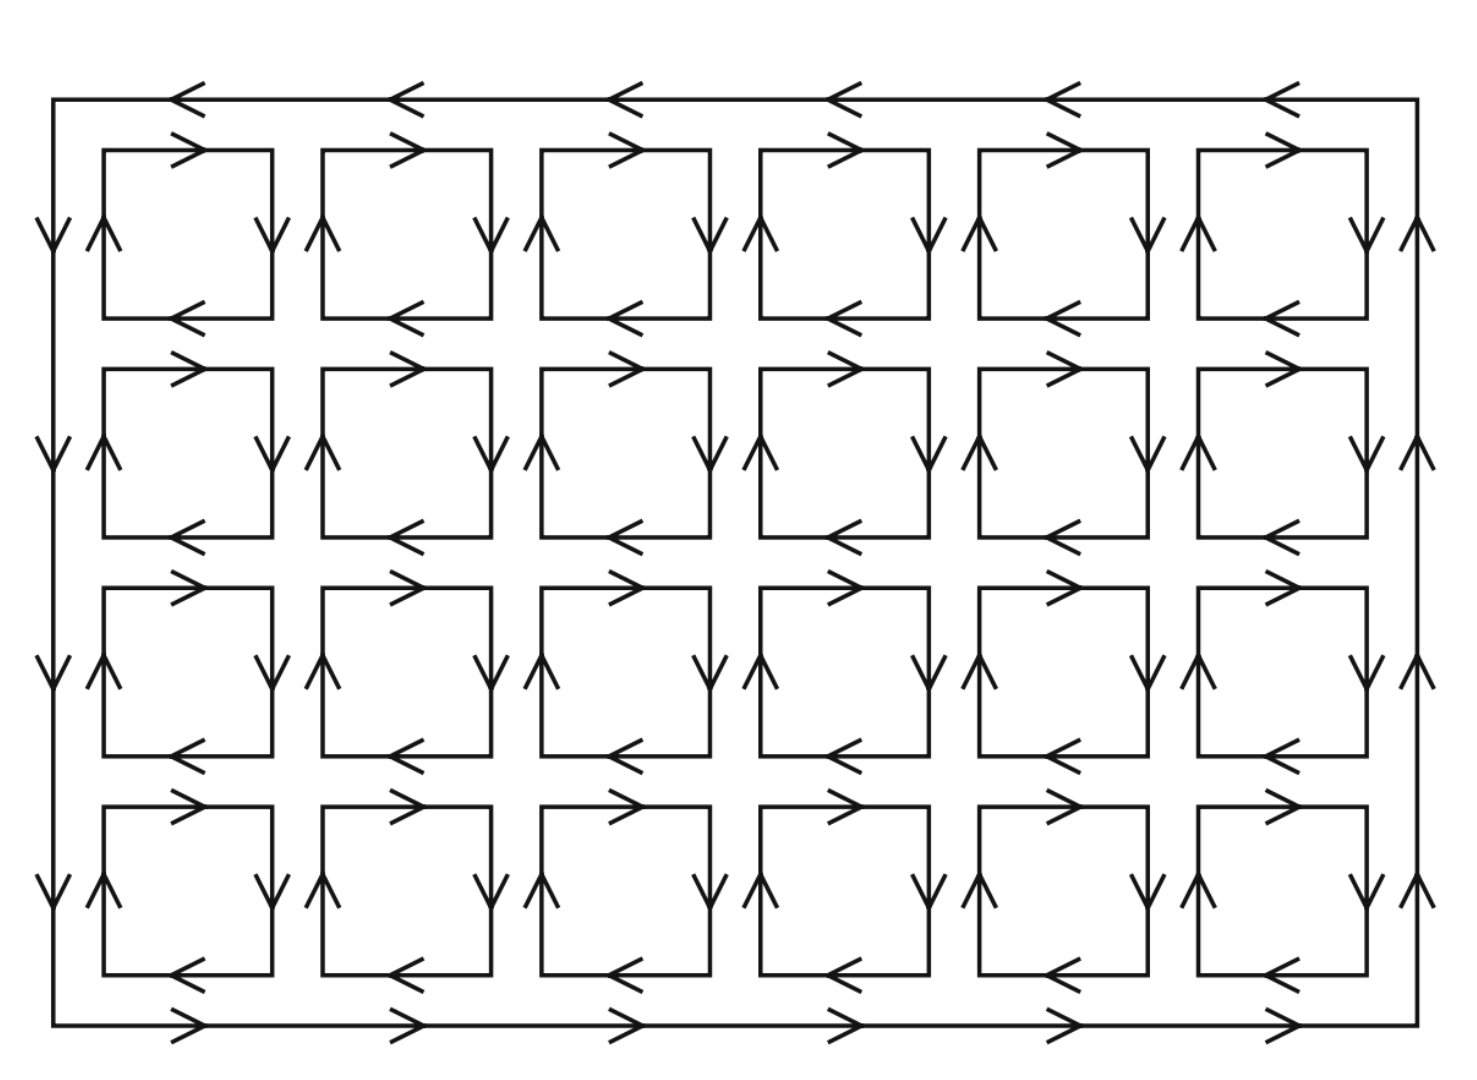
\includegraphics[scale=0.12]{IMG_DA3FC766B162-1.jpeg}
\end{figure}

Then,
\begin{align}
    \int D[\sigma]\prod_{l\in C}\sigma(l)e^{-S}&=(e^{-\beta}\cosh{\beta})^{N^2}(\tanh{\beta})^{Ar[C]}
\end{align}
Therefore,
\begin{align}
    \braket{\prod_{l\in C} \sigma(l)}&=\frac{(e^{-\beta}\cosh{\beta})^{N^2}(\tanh{\beta})^{Ar[C]}}{(e^{-\beta}\cosh{\beta})^{N^2}}\\
    &=(\tanh{\beta})^{Ar[C]}\\
    &=e^{Ar[C]\ln{\tanh{\beta}}}\\
    \Aboxed{\braket{\prod_{l\in C} \sigma(l)}&=e^{-f(\beta)Ar[C]}}
\end{align}
where
\begin{align}
    f(\beta)=-\ln{\tanh{\beta}}.
\end{align}


In our numerical calculation, the beta, $\beta=0.3$, so
\begin{align}
    \Aboxed{f_{\text{analytical}}(\beta)=-\ln{\tanh{0.3}}=1.23335831883}
\end{align}
\subsection{From Monte-Carlo simulation}
    From the lattice Monte Carlo simulation, we got the expected value from the analytical solution
    \begin{align}
    \Aboxed{f_{\text{numerical}}(\beta)=1.2334\pm0.0049}\checkmark
    \end{align}
    \begin{figure}[h!]
        \centering
        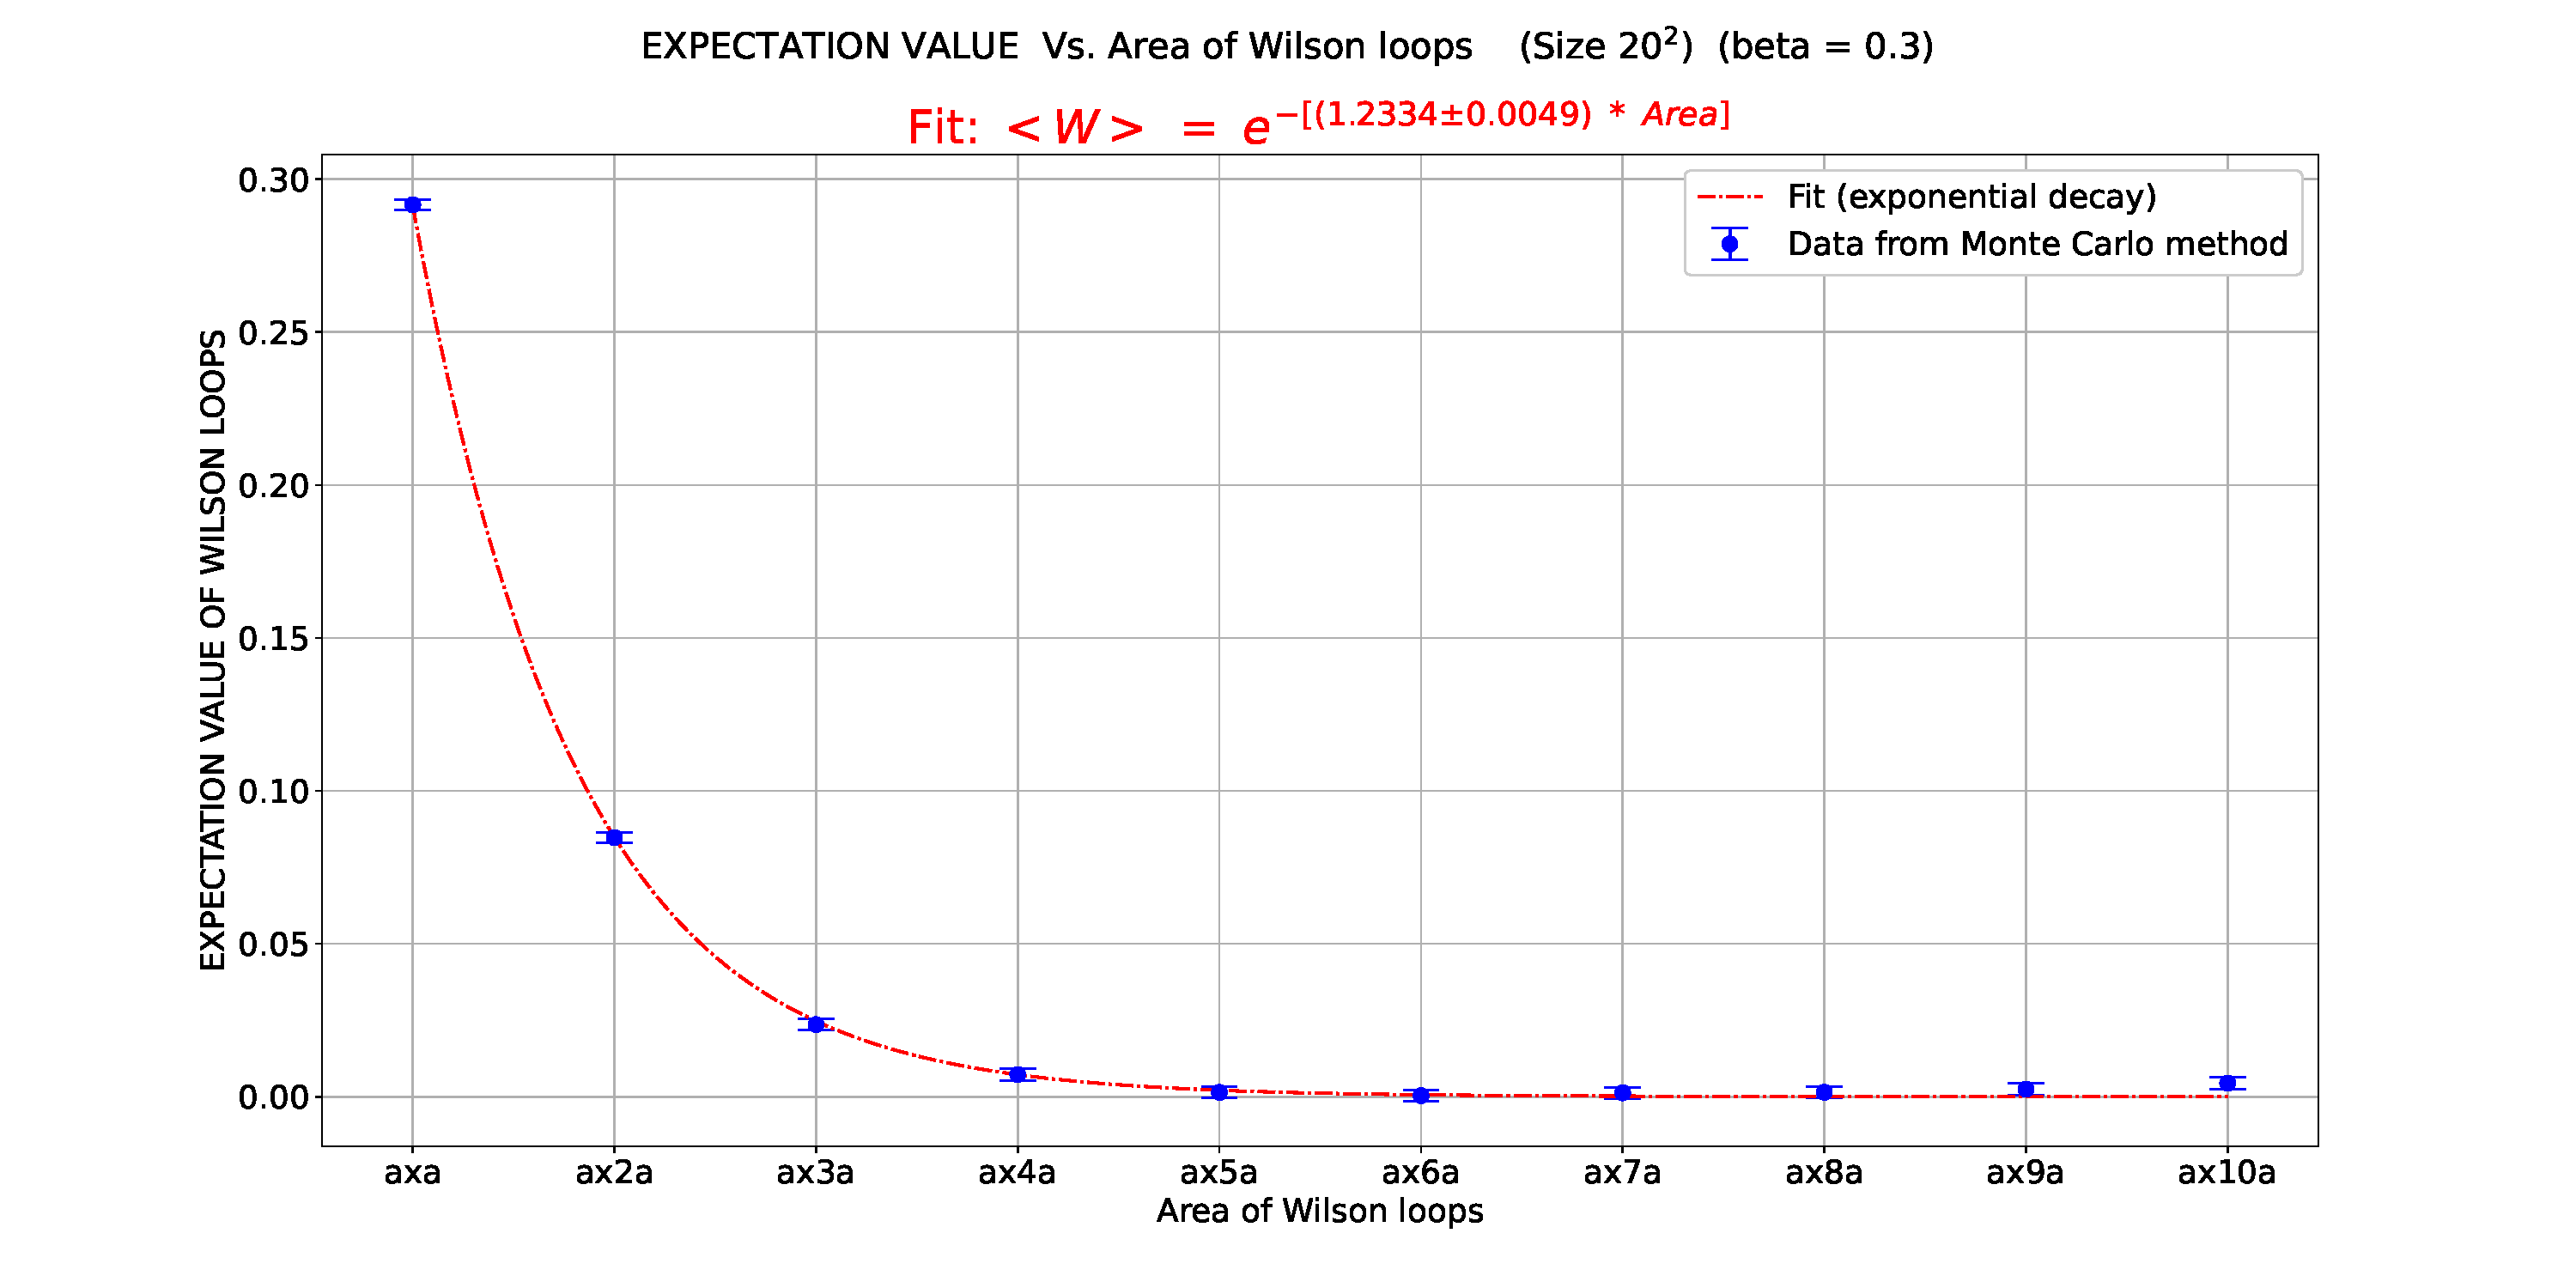
\includegraphics[scale=0.3]{arealawz2.pdf}
        \caption{Expectation value of Wilson loops - Monte Carlo simulations of $\mathbb{Z}_2$ lattice gauge theory $(1+1)$ }
        \label{fig:enter-label}
    \end{figure}

\pagebreak
\section{Other Interesting Calculations in Higher Dimensions}
All other interesting calculations from higher dimensional $\mathbb{Z}_2$ Monte Carlo simulations are archived in a GitHub repository: \href{https://github.com/Hariprashad-Ravikumar/Z2_LatticeGauge_Monte_Carlo_Simulation}{\texttt{github.com/Hariprashad-Ravikumar/Z2\_LatticeGauge\_Monte\_Carlo\_Simulation}}



\end{document}
